\chapter{Stability of fixed points}
Now we would like to begin to explore the behavious of dynamical systems around fixed points. This will allow us to find out if we should expect to observe a fixed state, and to understand what happens if we perturb the system away from this fixed state.
\section{Basic definitions}
Consider
\begin{align}
	\dot{ \bm{x}}=f( \bm{x},t),\  \bm{x} \in \mathbb{R}^{n},\ f\in C^{1}.
\end{align}
Assume that $ \bm{x}=0$ is a fixed point, i.e. $f(\bm{0},t) = \bm{0}$ for all $t \in \mathbb{R}$. If the fixed point is originally at $\bm{x}_0\neq \bm{0}$, shift it to zero by letting $\tilde{ \bm{x}}:= \bm{x}- \bm{x}_0$, therefore 
\begin{align}
	\dot{\tilde{ \bm{x}}} = \dot{ \bm{x}} = f( \bm{x}_0 + \tilde{ \bm{x}}, t) = \tilde{f}(\tilde{ \bm{x}}, t).
\end{align}
We would like to understand how the dynamical system behaves near its equilibrium state. To this end we introduce the following definitions.
\begin{definition}[Lyapupnov Stability]
	$ \bm{x}=\bm{0}$ is stable if for all $t_0$, for all $\epsilon>0$ small enough, there exists a $\delta=\delta(t_0, \epsilon)$, such that for all $ \bm{x}_0 \in \mathbb{R}^{n}$ with $\| \bm{x}_0\| \leq \delta$, we have 
	\begin{align}
		\left \|  \bm{x}(t;t_0,  \bm{x}_0) \right\| \leq \epsilon \quad \forall t \geq t_0.
	\end{align}
\begin{figure}[h!]
	\centering
	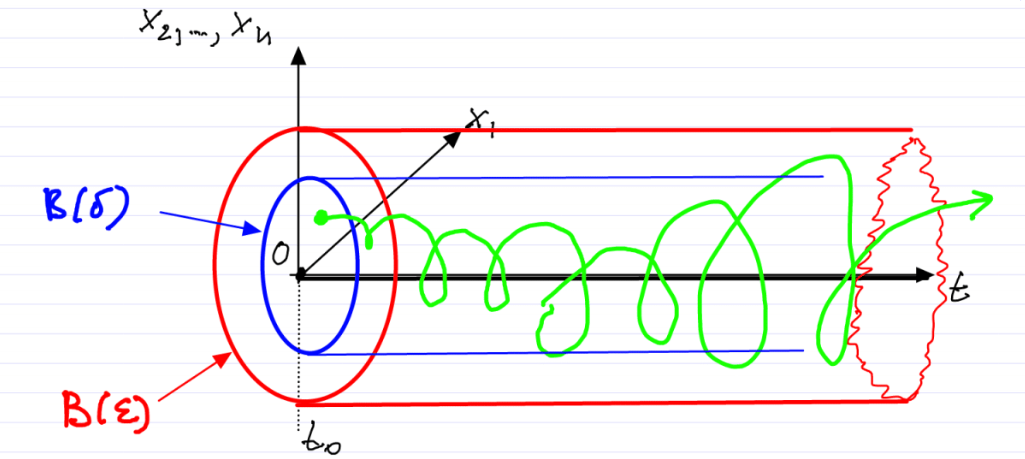
\includegraphics[width=0.7\textwidth]{figures/ch2/1lyapunov_stability.png}
	\caption{An example such a $\delta$, $B(r)$ represents the $n$-dimensional ball of radius $r$.}
	\label{fig:lyapunov_stability_def}
\end{figure}
\end{definition}

\begin{ex}[Stability of lower  equilibrium of the pendulum]
	Recall the equation of motion of the pendulum $\ddot{\varphi} + \sin(\varphi) = 0$, that we transform into a first order ODE by setting $x_1 = \varphi$ and $x_2 = \dot{\varphi}$ to obtain
	\begin{align}
		\begin{dcases}
		\dot{x}_1 = x_2 \\
	\dot{x}_2 = -\sin(x_1).
		\end{dcases}
	\end{align}
	For small $\epsilon>0$, this geometric procedure gives a $\delta(\epsilon)>0$ such that the definition of stability is satisfied for $ \bm{x}=0$. We can see in Fig. \ref{fig:pend_lower_stability}  that for any point chosen within the blue circle, it's trajectory remains within the red circle for all time (cf. Fig. \ref{fig:lyapunov_stability_def}. Therefore $ \bm{x}=0$ is (Lyapunov) stable.
	\begin{figure}[h!]
		\centering
		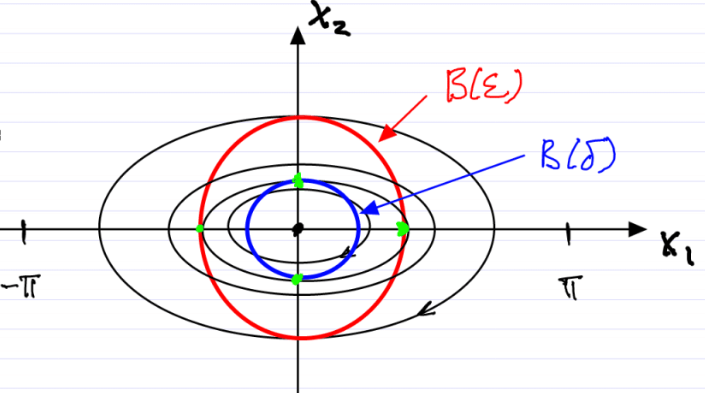
\includegraphics[width=0.5\textwidth]{figures/ch2/2pendulum_stability.png}
		\caption{Stability of lower equilibrium for the pendulum, here $0<\epsilon<\pi $.}
	\label{fig:pend_lower_stability}
	\end{figure}
\end{ex}

\begin{definition}[Asymptotic stability]
	The fixed point $ \bm{x}=0$ is \emph{asymptotically stable} if
\begin{enumerate}
	\item it is stable,
	\item for all $t_0$, there exists $\delta_0(t_0)$ such that for every $ \bm{x}_0$ with $\|  \bm{x}_0 \| \leq \delta_0$ we have
		\begin{align}
			\boxed{\lim_{t\to \infty }  \bm{x}(t; t_0,  \bm{x}_0) = 0.}
		\end{align}
\end{enumerate}
\begin{figure}[h!]
	\centering
	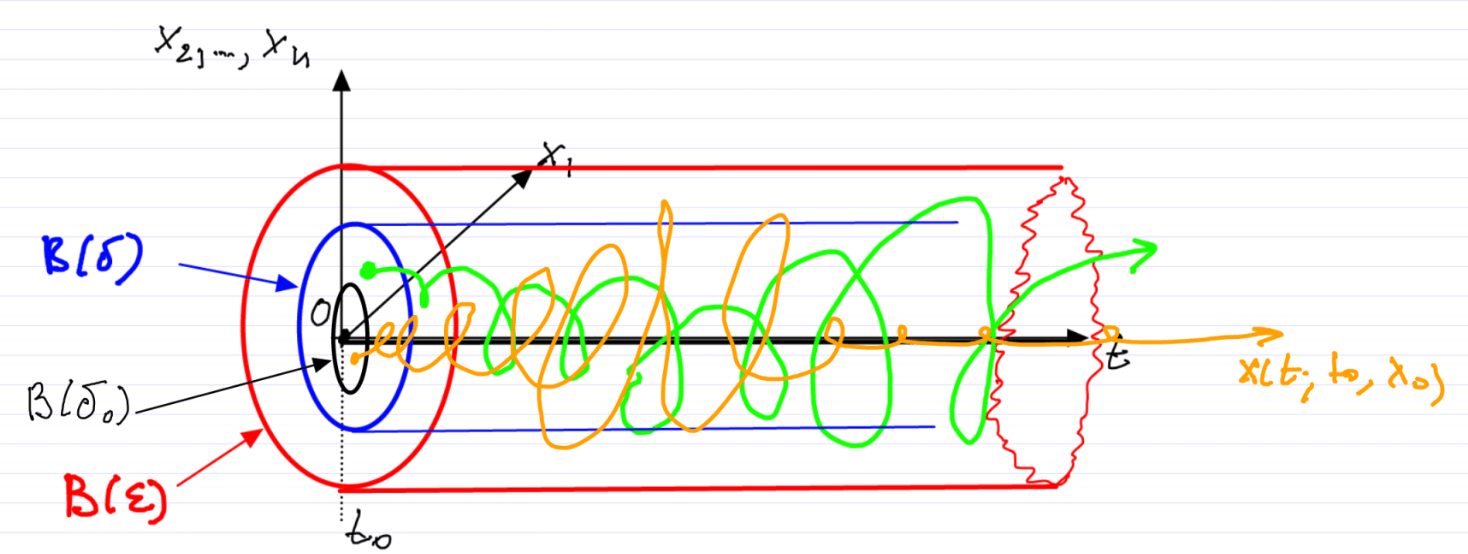
\includegraphics[width=0.7\textwidth]{figures/ch2/3asymp_stability.png}
	\caption{An example for an asymptotically stable fixed point (black trajectory).}
\end{figure}
\end{definition}

\begin{definition}[Domain of attraction] 
	The \emph{domain of attraction} is the set of all $ \bm{x}_0$'s for which
	\begin{align}
		\boxed{\lim_{t\to \infty } \bm{x}(t;t_0,  \bm{x}_0)=0. }	
	\end{align}
	
\end{definition}

\begin{ex}[Damped pendulum]
	We have the equation of motion with the linear damping coefficient $c$
	\begin{align}
		\ddot{\varphi} + c \dot{\varphi} + \sin(\varphi) = 0,\quad c>0.
	\end{align}
	Transforming into a first-order ODE with $x_1 = \varphi$ and $x_2 = \dot{\varphi}$ gives
	 \begin{align}
		\begin{dcases}
		\dot{x}_1 = x_2\\ \dot{x}_2 = -cx_2 - \sin(x_1).
		\end{dcases}
	\end{align}
The total energy is given by
\begin{align}
	E = \frac{1}{2}x_2^2 + \left( 1 - \cos(x_1) \right). 
\end{align}
Further we have the rate of energy change
\begin{align}
\frac{d}{dt} E(x_1(t), x_2(t)) = x_2 \left(\dot{x}_2 + \sin(x_1) \right) = -c x_2^{2}.
\end{align}
\begin{figure}[h!]
	\centering
	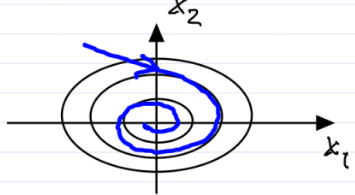
\includegraphics[width=0.35\textwidth]{figures/ch2/4damped_pendulum.png}
\end{figure}

Therefore, along trajectories energy decreases monotonically. By the $C^0$ dependence of the trajectory on initial conditions, the trajectories remain close to the undamped oscillations for small $c>0$. We conclude that trajectories are inward spirals for a small dissapation $c>0$ small. The fixed point $ \bm{x}=0$ is still Lyapunov stable, but asymptotic stability does not yet follow (is the limit of $ \bm{x}(t)$ equal to 0?).
\begin{remark}[LaSalle's invariance principle]
	This conclusion follows rigorously from LaSalle's invariance principle, namely if we assume that $\dot{ \bm{x}}=f( \bm{x})$, $f \in C^1$, and that there exists a $V\in C^1$ with 
	\begin{align}
		\dot{V} = \frac{dV( \bm{x}(t))}{dt} \leq 0.	
	\end{align}
	Then the set of accumulation points for any trajectory is contained in the set of trajectories that stay within the set $I=\{ \bm{x} \in \mathbb{R}^{n}:\ \dot{V}( \bm{x}) = 0\}$.
\end{remark}
\end{ex}

\begin{ex}[]
	Consider the following dynamical system in polar coordinates, i.e. $r\cos(\theta) = x$ and $r \sin(\theta) = y$,
	\begin{align}
		\begin{dcases}
			\dot{r} = r(1-r) \\ \dot{\theta} = \sin^2\left( \frac{\theta}{2} \right).
		\end{dcases}
	\end{align}
	Note that $r=0$ is a fixed point, the set $r=1$ is an invariant circle, and the set $\theta=0$ is an invariant set. An invariant set is a set such that if the dynamical system is started on the set, it remains in the set for all time. Examining the radial evolution reveals that the equation of motion decouples. We see that $\dot{\theta}\geq 0$, so rotation is either positive or null.
	\begin{figure}[h!]
		\centering
		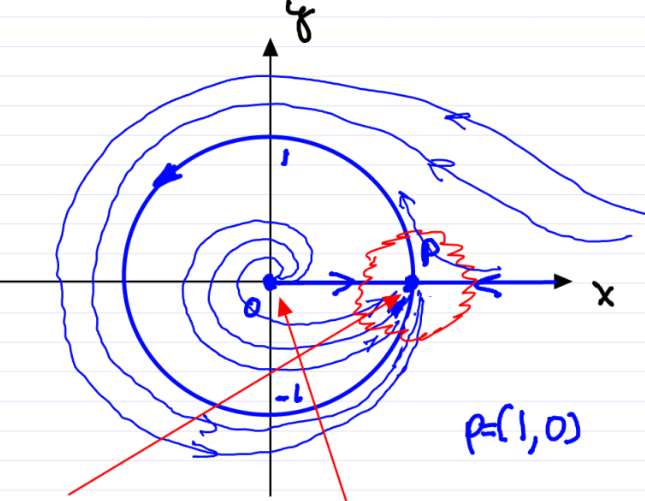
\includegraphics[width=0.5\textwidth]{figures/ch2/5polar_cds.png}
		\caption{Phase portrait of the dynamical system, with the red arrows pointing to the two unstable equilibria.}
	\end{figure}

	However, we have that $p=(1,0)$ is an example of an attractor: a set with an open neighborhood of points that all approach the set as $t\to \infty $.	
\end{ex}

\begin{definition}[Invariant set]
	The set $S \subset P$ is an \emph{invariant set} for the flow map $F^{t}:P \to P$ if $F^{t}(S) =S$ for all $t \in \mathbb{R}$.
\end{definition}

\begin{definition}[Unstable point]
	A fixed point $ \bm{x}=0$ is unstable if it is not stable.
\end{definition}

\begin{remark}[]
	We can negate a mathematical statement by using the reverse relational operators outside the statements involving these operators i.e. $ \exists \to \forall $ and $\forall \to \exists $. For example we have for continuity $\forall \epsilon\ \exists \delta:\  \|f( \bm{x}) - f( \bm{y}) \| < \epsilon$ if $ \| \bm{x}- \bm{y} \|<\delta$, meanwhile for discontinuity we have  $\exists \epsilon:\ \forall \delta:\  \|f( \bm{x}) - f( \bm{y}) \| \geq  \epsilon$ for $ \| \bm{x}- \bm{y} \|< \delta$.

	In our case for stability we have
	\begin{align}
		\forall \epsilon,t_0: \quad \exists \delta>0: \quad \forall  \bm{x}_0  \textrm{ with }  \| \bm{x}_0 \| < \delta: \quad  \| \bm{x}(t) \|\leq \epsilon \quad \forall t\geq t_0.
	\end{align}
Meanwhile for instability 
\begin{align}
	\exists \epsilon,t_0:\quad \underbrace{\forall \delta>0}_{ \textrm{``for arbitrarily small"} }:\quad \exists  \bm{x}_0  \textrm{ with }  \| \bm{x}_0 \|<\delta: \quad  \| \bm{x}(t) \|>\epsilon \quad \underbrace{\exists t\geq t_0}_{ \textrm{``for some"} }.
\end{align}
This negation is demonstration in Fig. \ref{fig:instable_def}
\begin{figure}[h!]
	\centering
	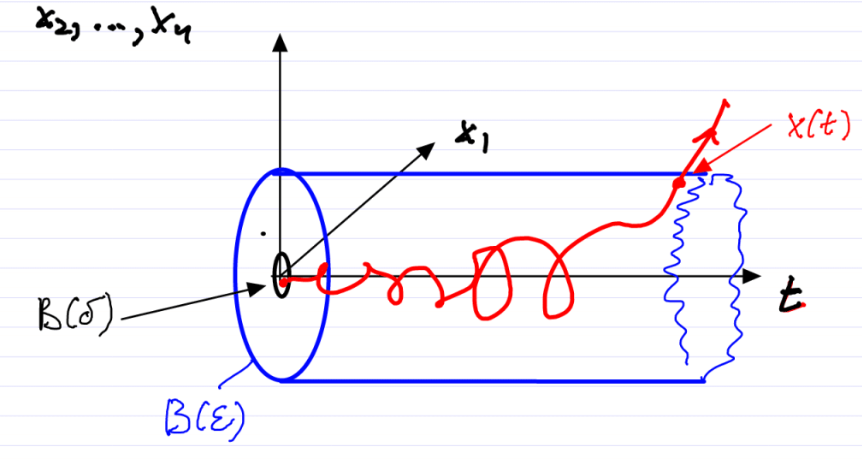
\includegraphics[width=0.5\textwidth]{figures/ch2/6unstable_def.png}
	\caption{Example of an unstable fixed point, with the red trajectory representing a trajectory starting arbitraritly close to the fixed point, leaving a given $\epsilon$-ball.}
	\label{fig:instable_def}
\end{figure}
\end{remark}

\begin{remark}[]
	By $C^0$ dependence of trajectories on initial conditions, if $ \bm{x}(t;t_0, \bm{x}_0)$ leaves $B(\epsilon)$, then for $\tilde{ \bm{x}}_0$ close enough to $ \bm{x}_0$, $ \bm{x}(t;t_0,\tilde{ \bm{x}}_0)$ also leaves $B(\epsilon)$. Since this is true on an open set around $\bm{x}_0$, the measure of such trajectories in nonzero, the instability is observable!
\end{remark}

\begin{ex}[Unstable fixed point of pendulum]
	In constrast, we can have that infinitely many trajectories converge to the fixed point, yet it is still unstable. In fact, the converging trajectories form a measure-zero set, thus the stability near the unstable equilibrium is unobservable.
	\begin{figure}[h!]
		\centering
		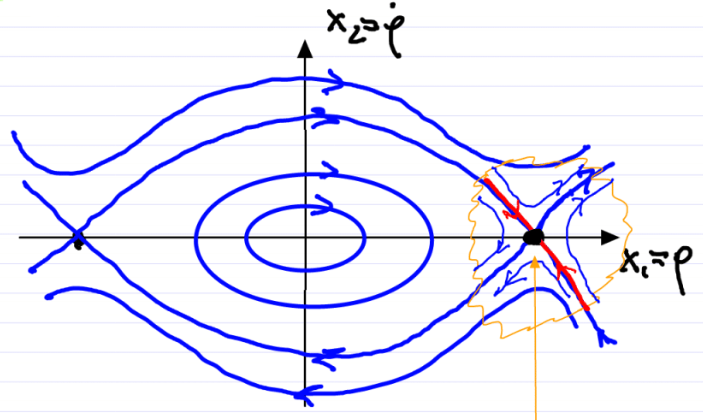
\includegraphics[width=0.6\textwidth]{figures/ch2/7unstable_pendulum.png}
		\caption{The phase portrait around the unstable fixed point of the pendulum, with the stable trajectories (red).}
	\end{figure}
	
\end{ex}
\newpage
\section{Stability based on linearization}
We would like to derive a more general method to analyze the stability of fixed points, thus we try to simplify our system around the fixed point and discover what this can tell us about the full (unsimplified) system. In the following section we shall always assume that our system is autonomous. We will have the following setup
\begin{align*}
	\dot{ \bm{x}}=f( \bm{x}),\quad f\in C^1,\quad  \bm{x}=
	\begin{pmatrix}
		x_1\\ \vdots \\ x_n
	\end{pmatrix}\in \mathbb{R}^{n}, \quad 
	\bm{p} = 
\begin{pmatrix}
	p_1 \\ \vdots \\ p_n 
\end{pmatrix}
\in \mathbb{R}^{n}. \numberthis \label{eq:star}
\end{align*}

